\chapter{Using the VSDT in ILIas}

% XXX am Ende noch andere Teile voruebergehend auskommentieren, die fuer ILIas
% weniger relevant sind (kommt da ueberhaupt wesentlich was zusammen?)
% - BPEL- und STP-Trafo-Zeugs (oder Trafo-Zeugs allgemein?)
% - JIAC-Node-Plugin?
% - Layout-Algorithmus (kann evtl. generell weg, oder in nen Anhang)

% Intro VSDT in ILIas (von Silvan, aus dem Meilenstein 2)
In order to create processes for managing the smart grid environment, a
corresponding development environment is adopted for better process creation and
-improvement.  One part of this environment is the process oriented development
of services for the SmaGriM system.  The main elements for this are services that
are provided as well defined functionalities by a service provider, in order to
allow service consumers to use those functionalities.  Such services can be
combined into processes that define concrete combinations of service calls, thus
realizing more complex functionalities.  Such processes are also called service
compositions and provide an easy to read yet powerful modeling approach for the
required grid management functionalities.

% Intro Prozess-Simulation (von Silvan, aus dem Meilenstein 2)
The ILIas system allows for extensive testing of services and processes developed
for the SmaGriM platform.  Simulations that are used to predict the behavior of
the grid to specific actions can also be used to test the effects of new or changed
implementations in what-if simulation scenarios.  Such scenarios are realized as
extended test cases by defining a test grid with known behavior, simulating new
services and processes in this scenario and comparing the simulation results to
the expected behavior of the grid.  This allows assessing the effects of changes
in a very concise procedure reducing overall testing efforts.

% Outline dieses Kapitels
Using the Visual Service Design Tool (VSDT), those processes can be modeled,
simulated (tested) using the SmaGriM simulation and finally be deployed to the
system.  In the following Sections, we will describe the general process of using
the VSDT in the ILIas project and then provide details about how to simulate the
process models prior to deploying them to the live system.


%%%%%%%%%%%%%%%%%%%%%%%%%%%%%%%%%%%%%%%%%%%%%%%%%%%%%%%%%%%%%%%%%%%%%%%%%%%%%%%%
%%  The ILIas Development Process                                             %%
%%%%%%%%%%%%%%%%%%%%%%%%%%%%%%%%%%%%%%%%%%%%%%%%%%%%%%%%%%%%%%%%%%%%%%%%%%%%%%%%

\section{The ILIas Development Process}

% verschiedene Rollen und Entwicklungsphasen beschreiben
Two main roles can be identified in the ILIas development process:  First, there
is the \emph{process engineer}, whose role is (a) developing and providing
different basic services to be orchestrated to complex processes in the process
diagram, and (b) creating such orchestrations for handling individual emergency
situations, such as power outages, and deploying them on a repository for later
use.  In both cases, the process engineer's creations have to be certified before
being put to productive use.  And second, there is the \emph{SmaGriM Operator},
monitoring the system, whose job in case of an emergency is to select a suitable
process from the repository, adapt it to the needs of the situation, test it in
the simulation, and finally deploy it to the actual system.  Finally, there are
a number of agents and other computer systems involved in the process, such as
the process repository, or the simulation (Figure~\ref{fig:ilias-use-cases}).

\begin{figure}[ht]
	\centering
	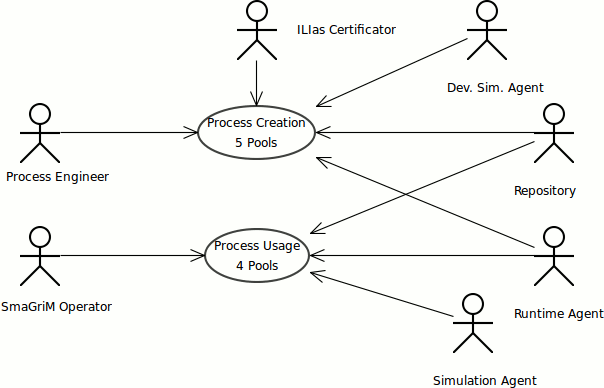
\includegraphics[width=.5\textwidth]{ilias/bpmn_ilias-1.png}
	\caption{ILIas Use Cases}
	\label{fig:ilias-use-cases}
\end{figure}

In the following we will give a short description of the two main use cases
(regarding the VSDT) in the scope of the ILIas project: \emph{Process Creation}
and \emph{Process Usage}.

%%%%%%%%%%%%%%%%%%%%%%%%%%%%%%%%%%%%%%%%%%%%%%%%%%%%%%%%%%%%%%%%%%%%%%%%%%%%%%%%

\subsection{Process Engineer: Process Creation}

The use case of \emph{Process Creation} is laid out in Figure~\ref{fig:ilias-proc-creation}.

\begin{figure}[ht]
	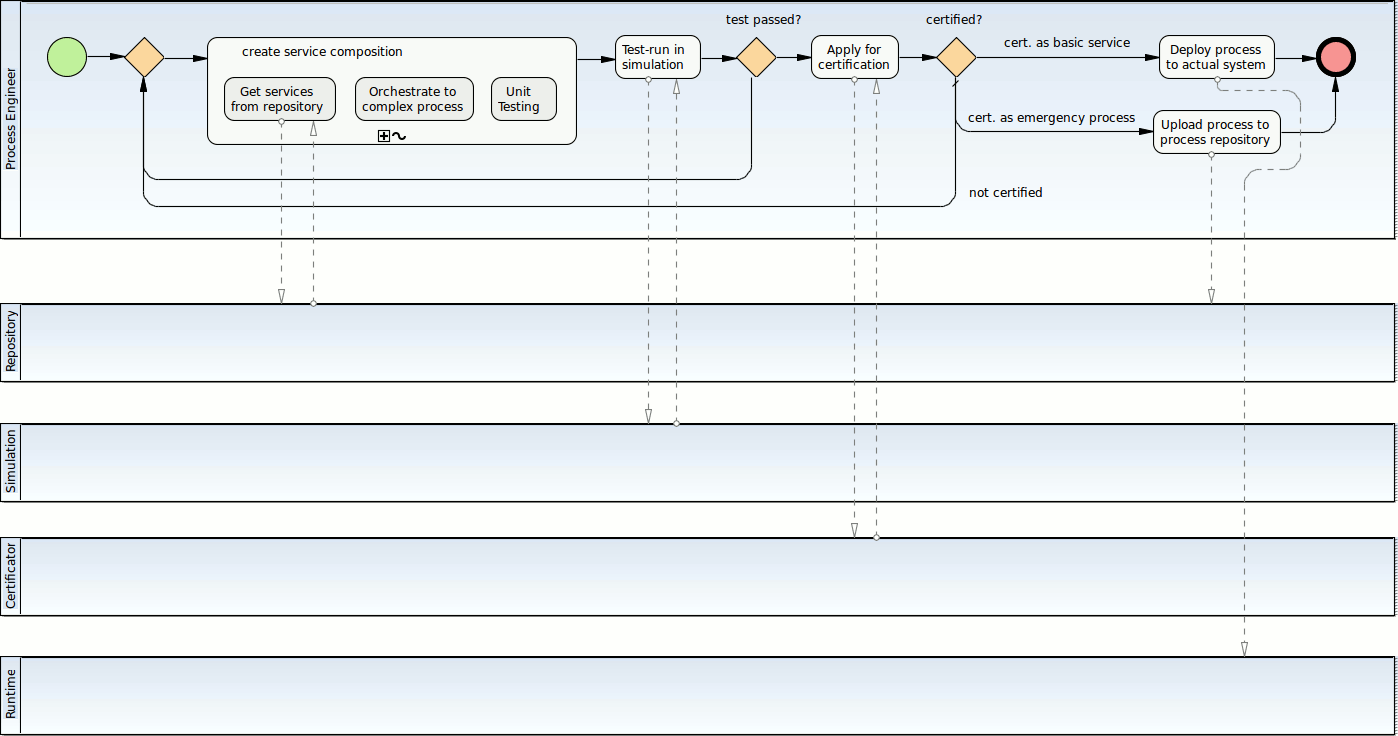
\includegraphics[width=\textwidth]{ilias/bpmn_ilias-2.png}
	\caption{ILIas Use Case \emph{Process Creation}}
	\label{fig:ilias-proc-creation}
\end{figure}

The actual process engineering consists of three activities: retrieving basic
services from the repository, orchestrating those service to a meaningful, complex
process, and testing the process or individual parts of this.  These tasks can be
carried out using the generic process modeling assistants provided by the VSDT.

Once the functionality of the process itself has been tested, the process is
deployed on the simulation environment for testing how the process integrates
into the ILIas environment.\footnote{For this purpose, the developer uses a
separate simulation, and not the one used by the SmaGriM Operator for testing
compensatory processes in case of an emergency.} Next, the process has to be
certified, to ensure that only thoroughly tested and simulated processes, which
do not do harm to the system, are deployed.  If either the simulation or the
certification fail, the process engineer has to go back to the drawing board
and rework the process.

Finally, certified processes can be deployed.  There are two possibilities:
Either, the process is deployed as a basic service, which means that it can be
reused as part of another process; in this case the process is deployed to the
runtime, so it can be invoked on demand.  Or the process is deployed as an
emergency process, for use only in special emergency situations; in this case the
process is deployed to the process repository, from where it can be retrieved
when needed.


%%%%%%%%%%%%%%%%%%%%%%%%%%%%%%%%%%%%%%%%%%%%%%%%%%%%%%%%%%%%%%%%%%%%%%%%%%%%%%%%

\subsection{SmaGriM Operator: Process Usage}

The use case of \emph{Process Usage} is depicted in Figure~\ref{fig:ilias-proc-usage}.

\begin{figure}[ht]
	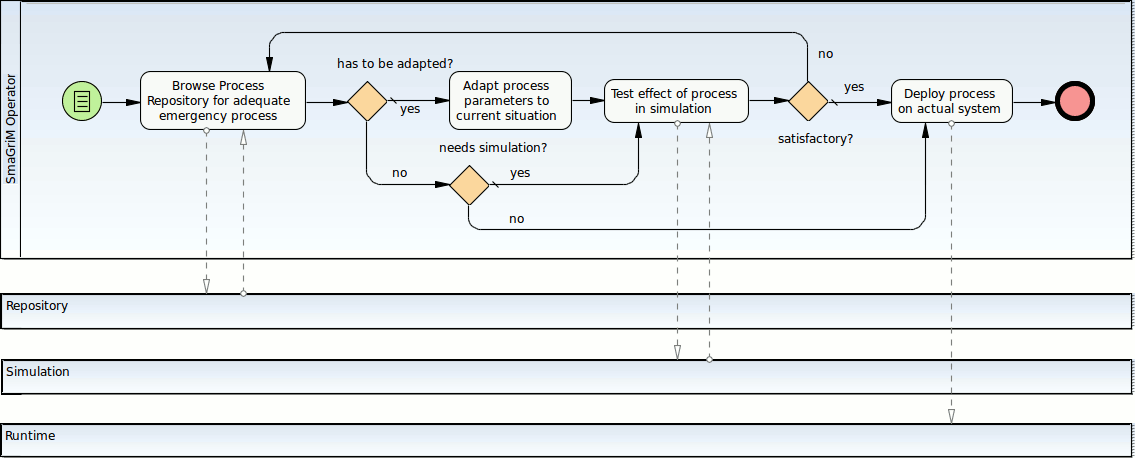
\includegraphics[width=1\textwidth]{ilias/bpmn_ilias-3.png}
	\caption{ILIas Use Case \emph{Process Usage}}
	\label{fig:ilias-proc-usage}
\end{figure}

This process is executed in case of an unexpected power outage or a similar
emergency event.  After assessing the situation, the SmaGriM Operator looks for
an adequate compensatory process for handling this kind of event in the process
repository.  In case the process has parameters, those are adapted to the current
situation (e.g. some sort of threshold, or IDs).

Afterwards, the process (with the selected parameter configuration) is tested in
a simulation precisely mirroring the current state of the grid.\footnote{It is
also possible that the process does not require to be simulated, which may be
necessary for emergencies demanding for very short response times.  Determining
this property will be part of the certification.} If the process does not show
the desired results in the simulation, the operator has to select a different
process or adapt the parameters; otherwise, the process can be deployed to the
runtime for countering the emergency situation.


%%%%%%%%%%%%%%%%%%%%%%%%%%%%%%%%%%%%%%%%%%%%%%%%%%%%%%%%%%%%%%%%%%%%%%%%%%%%%%%%
%%  Testing Processes in the ILIas Simulation                                 %%
%%%%%%%%%%%%%%%%%%%%%%%%%%%%%%%%%%%%%%%%%%%%%%%%%%%%%%%%%%%%%%%%%%%%%%%%%%%%%%%%

\section{Testing Processes in the ILIas Simulation}

In the following we will provide a detailled description of those components of
the VSDT which have been created especially for the ILIas project, foremost the
\emph{Simulation View}, providing the connection to the agents running the
simulation.


\subsection{The ILIas Simulation View}

% Beschreibung des Views
The ILIas Simulation View provides an interface to the ILIas Simulation, where
newly created or adapted process models can be tested for suitability (see
Figure~\ref{fig:ilias-simview}).  The view provides a number of controls for
deploying the process model from the active editor window to the simulation, for
starting and stopping the simulation and for viewing the status of the simulation.

% TODO richtiges Bild erstellen und einbinden
\begin{figure}[ht]
	\centering
	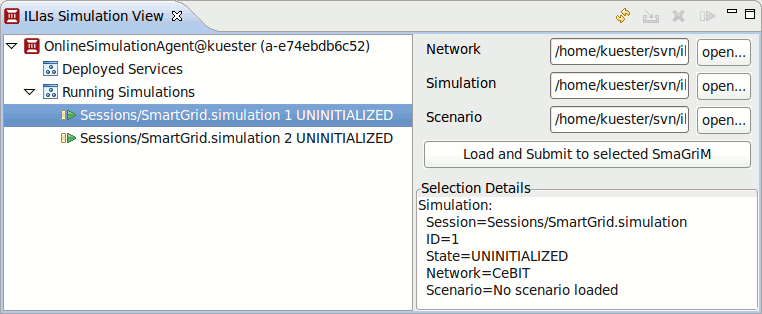
\includegraphics[width=.6\textwidth]{ilias/ilias-view_110725.png}
	\caption{ILIas Simulation View}
	\label{fig:ilias-simview}
\end{figure}

% Funktionsweise: Teil des Node-Plugins, Anbindung an ILIas-Agenten (?)
The Simulation View is based on the \emph{JIAC Node Plugin} (see Section
\ref{sec:user_jiac-node}), and the deployment mechanism is similar to that of the
\emph{Deployment View}, the only difference being that the processes can not be
deployed to arbitrary JIAC agents, but only to an ILIas Simulation Agent.

% Funktionsweise: JADL-Services und Service-Starter-Rules
Like for the regular deployment view, the processes are transformed to executable
JADL services and then deployed to an agent equipped with a JADL interpreter
running on the simulation node.  Additionally, besides the services also a number of
service starter rules are deployed to that agent, so that the individual JADL
services are started just in the way stated by the processes' start events.


\subsection{Simulating Processes}
% Klick-Weg zum Simulieren eines Prozesses:
% Welche Bedingungen muessen erfuellt sein, was muss alles eingestellt werden, etc.

% TODO detaillierte Beschreibung

\subsection{Deploying and Executing Processes}
% Nach der Simulation: Deployment auf 'Produktiv-Umgebung' (geht das auch ueber
% die Simulation View, oder verwendet man hierfuer wieder die Deployment View?)




